\begin{frame}{}
    \transcover
\end{frame}

\begin{frame}{}
    \transfade
    \begin{columns}
    \column{0.4\textwidth}
    \begin{itemize}
        \item<1->[$\blacksquare$] Kahn's Algorithm
        \item<2->[$\blacksquare$] BFS
        \item<3->[$\blacksquare$] {$O(|V|+|E|)$}
    \end{itemize}
    \column<1->{0.6\textwidth}
    \begin{algorithm}[H]
    % \algsetup{linenosize=\tiny}
    \begin{algorithmic}[1]
    \small
    \Procedure{TopoSort}{$G$} 
    \State create a list $L$
    \State create a queue $Q$
    \ForEach {vertex $v \in G$}
    \If{the indegree of $v = 0$}
    \State put v into the $Q$
    \EndIf
    \EndFor
    \While{$Q$ is not empty}
    \State pop a vertex v out of $Q$
    \State add v to the end of $L$
    \ForEach {edge $(u,v) \in G$}
    \State decrement the indegree of u
    \If{the indegree of $u = 0$}
    \State put u into the $Q$
    \EndIf
    \EndFor
    \EndWhile
    \State \Return $L$
    \EndProcedure
    \end{algorithmic}
\end{algorithm}
    \end{columns}
\end{frame}

\begin{frame}{}
    \transcover
\end{frame}

\begin{frame}{}
    \transfade
    \color{black}
    \begin{figure}
    \centering
        \begin{tikzpicture}
        \node<1-3> (A) [vertex3] {\Large A};
        \node<1-3> (B) [vertex3, right of = A,xshift = 60] {\Large B};
        \node<1-3> (C) [vertex3, right of = A,xshift =20, yshift=-60] {\Large C};
        
        \node<4> (A) [vertex] {A \nodepart{lower} 1};
        \node<4> (B) [vertex, right of = A,xshift = 60] {B \nodepart{lower} 1};
        \node<4> (C) [vertex, right of = A,xshift =20, yshift=-60] {C \nodepart{lower} 1};
        \draw [arrow] (A) -- (B);
        \draw [arrow] (B) -- (C);
        \draw [arrow] (C) -- (A);
    \end{tikzpicture}
    \end{figure}
    \begin{block}{}<2->
            \centering
            \Large What is the topological order?
    \end{block}
    \begin{block}{}<3->
            \centering
            \color{red}
            \Huge Not possible :(
    \end{block}
\end{frame}

\begin{frame}{}
    \transfade
    \Large
    \begin{block}{}<1->
        \centering
        Topological sorting is applicable for Directed Acyclic Graph (DAG). 
    \end{block}
    %  \begin{block}{}<2>
    %     \centering
    %     What's wrong with cyclic graphs? 
    % \end{block}
\end{frame}


\setbeamercolor{background canvas}{bg=black}
\begin{frame}{}
    \transcover
\begin{tikzpicture}
     \draw[color=white,fill=white,transform canvas={xshift = 5cm, yshift=-0.5cm}] (0,0) rectangle (0.2,3);
\end{tikzpicture}
\begin{textblock}{5}(6.5,7.3)
\fontfamily{qhv}\selectfont
\Huge\color{white} \textbf{WHERE?}
\end{textblock}
\end{frame}
\setbeamercolor{background canvas}{bg=white}
\begin{frame}{}
    \transuncover
\end{frame}

\setbeamercolor{background canvas}{bg=white}
    \color{black}
    % \begin{block}{}<1->
    %     Let's say we have two tasks A and B. 
    % \end{block}
    % \begin{block}{}<3->
    %     Task A is prerequisite of Task B.
    % \end{block}

    \begin{textblock}{14}(1,2)
    \begin{itemize}
        \only<1-2> {
            \vfill \item<1->[$\blacksquare$] Let's say there are two nodes A and B.
            \vfill \item<2->[$\blacksquare$] And there is an edge from A to B, we can say that B is dependent on A
        }
        \item[$\blacksquare$]<3-> Focus on indegree (Number of incoming edges) in each node
        \item<4->[$\blacksquare$] Indegree represents dependency. B has 1, A has none.
        \item<5->[$\blacksquare$] A node can be visited only if it doesn't have any dependencies or we can say if the indegree is 0 
    \end{itemize}
    \end{textblock}

    \begin{textblock}{16}(0,7)
    \begin{figure}
    \centering
    \begin{tikzpicture}
        \node<1-2> (A) [vertex3] {\Large A};
        \node<1-2> (B) [vertex3, right of = A,xshift = 60] {\Large B};
        \draw<2-2> [arrow] (A) -- (B);
        
        \node<3-> (A) [vertex] {A \nodepart{lower} 0};
        \node<3-> (B) [vertex, right of = A,xshift = 60] {B \nodepart{lower} 1};
        \draw<3-> [arrow] (A) -- (B);

    \end{tikzpicture}
    % \begin{textblock}{16}(0,7.3)
    % \begin{tikzpicture}
    %     \node<5-> (T1) [yshift=0,xshift=0,red] {\Large \textbf{Indegree}};
    %     \draw<5->[arrow, draw=red] (T1.west) -|+ (-0.45,1.35);
    %     \draw<5->[arrow, draw=red] (T1.east) -|+ (0.45,1.35);
    %     % \path [->, draw=red]
    %     %     (T1.west) edge [bend left] (-1.5,1.3)
    %     %     (T1.east) edge [bend right] (1.5,1.3);
    % \end{tikzpicture}
    % \end{textblock}
    \end{figure}
    \end{textblock}
    

\begin{frame}{}
    \transcover
\end{frame}

\begin{frame}{}
\transfade
    \begin{textblock}{15}(1,2)
    \begin{itemize}
        \item[$\blacksquare$] Operation System deadlock detection.  
    \end{itemize}
    \end{textblock}
    \begin{textblock}{16}(0,4.4)
    \setbeamercovered{transparent}
    \begin{figure}
        \centering
        \begin{tikzpicture}[->, thick, >=stealth]
            \node(A) [vertex7, fill=blue!30]  {Process 1};
            \node(B) [vertex5, below of = A, xshift = -80, yshift = -15,fill=orange!30] {Resource 1};
            \node(C) [vertex5, below of = A, xshift = 80, yshift = -15,fill=orange!30] {Resource 2};
            \node(D) [vertex7, below of = A, xshift = 0, yshift = -60, fill=blue!30] {Process 2};
            
            
            \path (A) edge [bend right] node[anchor=east] {Waiting for} (B);
            \path (B) edge [bend right] node[anchor=east] {Assigned to} (D);
            \path (D) edge [bend right] node[anchor=west] {Waiting for} (C);
            \path (C) edge [bend right] node[anchor=west] {Assigned to} (A);
            
        \end{tikzpicture}
    \end{figure}
\end{textblock}
\end{frame}

\begin{frame}{}
    \transcover
\end{frame}

\begin{frame}{}
\transfade
    \begin{textblock}{15}(1,2)
    \begin{itemize}
        \item[$\blacksquare$] Course Schedule problem. 
    \end{itemize}
    \end{textblock}
    \begin{textblock}{16}(0,4)
    \setbeamercovered{transparent}
    \begin{figure}
        \centering
        \begin{tikzpicture}[->, thick, >=stealth]
            \node(A) [vertex5]  {CSE 309};
            \node(B) [vertex5, below of = A, xshift = 0, yshift = -15] {CSE 211};
            \node(C) [vertex5, right of = A, xshift = 50, yshift =  75] {CSE 101};
            \node(D) [vertex5, right of = A, xshift = 50, yshift =  40] {CSE 107};
            \node(E) [vertex5, right of = A, xshift = 50, yshift =  0] {CSE 203};
            \node(F) [vertex5, below of = E, xshift = 0, yshift =  -15] {CSE 207};
            \node(G) [vertex5, right of = E, xshift = 90, yshift =  0] {CSE 205};
            \node(H) [vertex5, right of = F, xshift = 50, yshift =  0] {CSE 305};
            \node(I) [vertex5, right of = F, xshift = 130, yshift =  0] {CSE 315};

            \draw (B) -- (A);
            \draw (C) -| (A);
            \draw (C) -- (D);
            \draw (D) -- (E);
            \draw (E) -- (F);
            \draw (G) -| (H);
            \draw (G) -| (I);        
        
        \end{tikzpicture}

    \end{figure}
\end{textblock}
\end{frame}

\begin{frame}{}
    \transfade
    \begin{textblock}{15}(1,2)
        \begin{itemize}
            \item[$\blacksquare$] Course Schedule problem. 
        \end{itemize}
    \end{textblock}
    
    \begin{textblock}{16}(0,5.5)
    \centering
    \begin{tikzpicture}[->, thick, >=stealth]
    \node(A) [vertex6]  {CSE 101};
    \node(B) [vertex6, right of = A, xshift = 15, yshift = 0] {CSE 107};
    \node(C) [vertex6, right of = B, xshift = 15, yshift =  0] {CSE 203};
    \node(D) [vertex6, right of = C, xshift = 15, yshift =  0] {CSE 207};
    \node(E) [vertex6, right of = D, xshift = 15, yshift =  0] {CSE 205};
    \node(F) [vertex6, right of = E, xshift = 15, yshift =  0] {CSE 211};
    \node(G) [vertex6, right of = F, xshift = 15, yshift =  0] {CSE 305};
    \node(H) [vertex6, right of = G, xshift = 15, yshift =  0] {CSE 309};
    \node(I) [vertex6, right of = H, xshift = 15, yshift =  0] {CSE 315}; 
    
    \draw (A) -- (B);
    \draw (B) -- (C);
    \draw (C) -- (D);
    \draw (A) --+ (0,1.5) -| (H);
    \draw (F) --+ (0,-1) -| (H);
    \draw (E) --+ (0,1) -| (G);
    \draw (E) --+ (0,-1.5) -| (I);
    \end{tikzpicture}
    \end{textblock}
\end{frame}


\begin{frame}{}
    \transcover
\end{frame}

\begin{frame}{}
\transfade
\begin{textblock}{16}(1,1.5)
    \begin{tikzpicture}

    \node<1->[inner sep=0pt] (b) at (0,4)
        {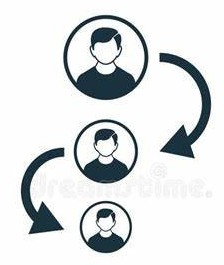
\includegraphics[width=.15\textwidth]{Simulation_souvik/Pictures/dependency.jpeg}};
    \node<1->[below of = b, yshift=-20]{Dependency resolution}; 
    
    \node<2->[inner sep=0pt] (f) at (5,4) {
\includegraphics[width=.18\textwidth]{Simulation_souvik/Pictures/workflow.png}};
    \node<2->[below of = f, yshift=-20]{Manufacturing workflow};  
      
    \node<3->[inner sep=0pt] (e) at (10,4)
        {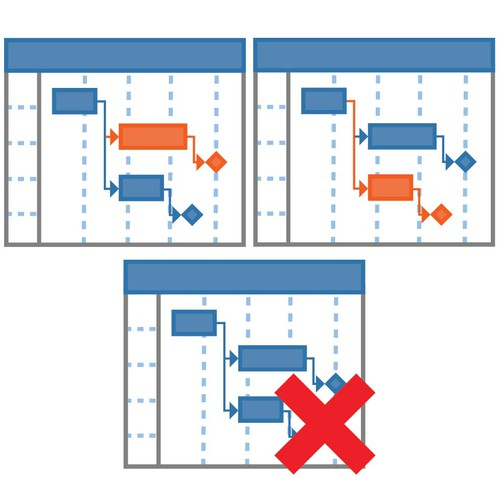
\includegraphics[width=.18\textwidth]{Simulation_souvik/Pictures/critical.jpeg}};
    \node<3->[below of = e, yshift=-20]{Critical path analysis};
    
    \node<4->[inner sep=0pt] (c) at (0,0.5)
        {
\includegraphics[width=.18\textwidth]{Simulation_souvik/Pictures/sentance.jpeg}};
    \node<4->[below of = c, yshift=-15]{Sentence ordering};   
    
    \node<5->[inner sep=0pt] (a) at (5,0.5)
        {
\includegraphics[width=.2\textwidth]{Simulation_souvik/Pictures/Task.png}};  
    \node<5->[below of = a, yshift=-15]{Task scheduling};
    
    \node<6->[inner sep=0pt] (d) at (10,0.5)
        {
\includegraphics[width=.18\textwidth]{Simulation_souvik/Pictures/data.jpeg}};
    \node<6->[below of = d, yshift=-15]{Data serialization};
\end{tikzpicture}
\end{textblock}
\end{frame}


% \begin{frame}{}
%     \begin{itemize}
%         \item[$\blacksquare$] Single Source Shortest Path in a DAG. \pause
%         \item[$\blacksquare$] Dependency resolution.\pause
%         \item[$\blacksquare$] Sentence Ordering. \pause
%         \item[$\blacksquare$] Critical Path Analysis. \pause
%         \item[$\blacksquare$] Scheduling jobs from given dependencies among Jobs. For example, if some job requires the dependency of some other job, then we can use topological sorting. \pause
%         \item[$\blacksquare$] Other applications like manufacturing workflows, data serialization and context-free grammar. \pause
%     \end{itemize}
% \end{frame}
